\chapter{Gradient Descent}
\section{Visualizing Gradient Descent}
\noindent
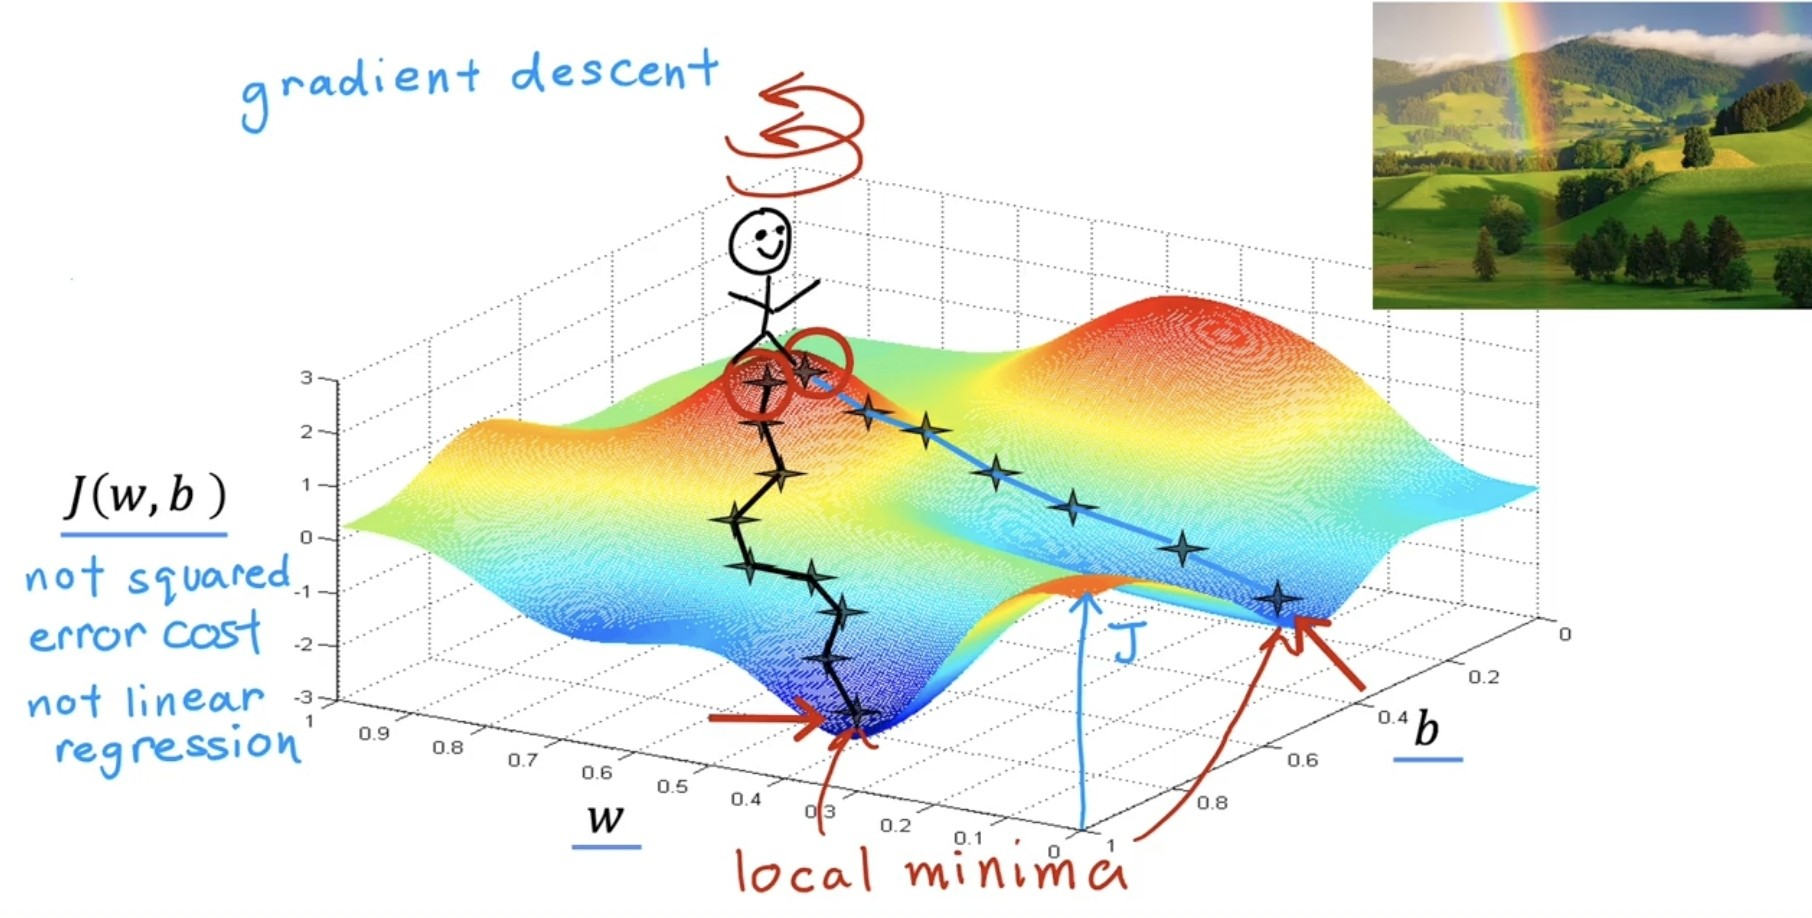
\includegraphics[width=\textwidth]{images/2.2_4}
\begin{notebox}
    Terminology: 
    local minimas, global minimas, saddle points
\end{notebox}

\section{Algorithm}
\begin{thmbox}{Gradient Descent Algorithm}{algorithm}
repeat until convergence
\begin{align}
    &w = w - \alpha \cdot \frac{\partial}{\partial w} J(w, b) \\
    &b = b - \alpha \cdot \frac{\partial}{\partial b} J(w, b)
\end{align}
\tcblower

\begin{minipage}{0.5\textwidth}
    \begin{itemize}
    \item note that $=$ represents assignment, not equality
    \item $\alpha$ is the learning rate
    \item It is important to \textbf{simutaniously} update $w$ and $b$
    \end{itemize}
    
    \begin{notebox}
        when $w > w_{min}$, the derivative is positive, so $w$ will decrease\par
        when $w < w_{min}$, the derivative is negative, so $w$ will increase
    \end{notebox}
\end{minipage}
\qquad
\begin{minipage}{0.4\textwidth}
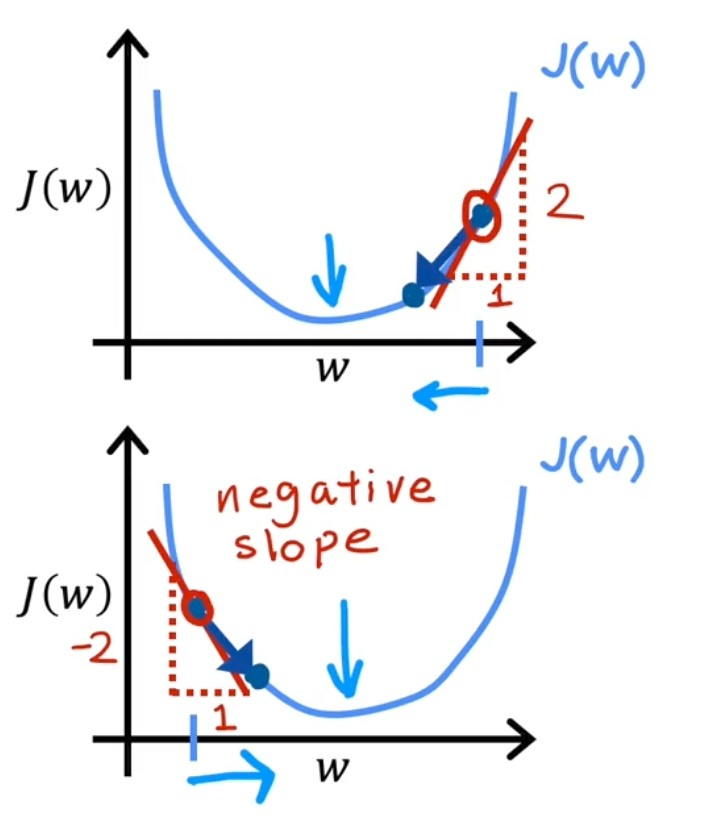
\includegraphics[width=\textwidth]{images/2.3_1}
\end{minipage}
\end{thmbox}

\subsection*{Learning Rate}
\noindent
\begin{minipage}{0.4\textwidth}
\includegraphics*[width=\textwidth]{images/2.3_2}
\end{minipage}
\begin{minipage}{0.6\textwidth}
\begin{enumerate}
    \item If the learning rate is too small, the algorithm will take a long time to converge\par
    \item If the learning rate is too large, %
    the algorithm may overshoot the minimum or even diverge.
\end{enumerate}
\end{minipage}

\begin{exbox}{local minima}{localminima}
    if the w eactly at the local minima, the derivative is 0,%
    the $w$ remains the same according to the equation so the algorithm will stop.
\end{exbox}

\subsection*{Why is it can reach local minima with fixed learning rate?}
\noindent
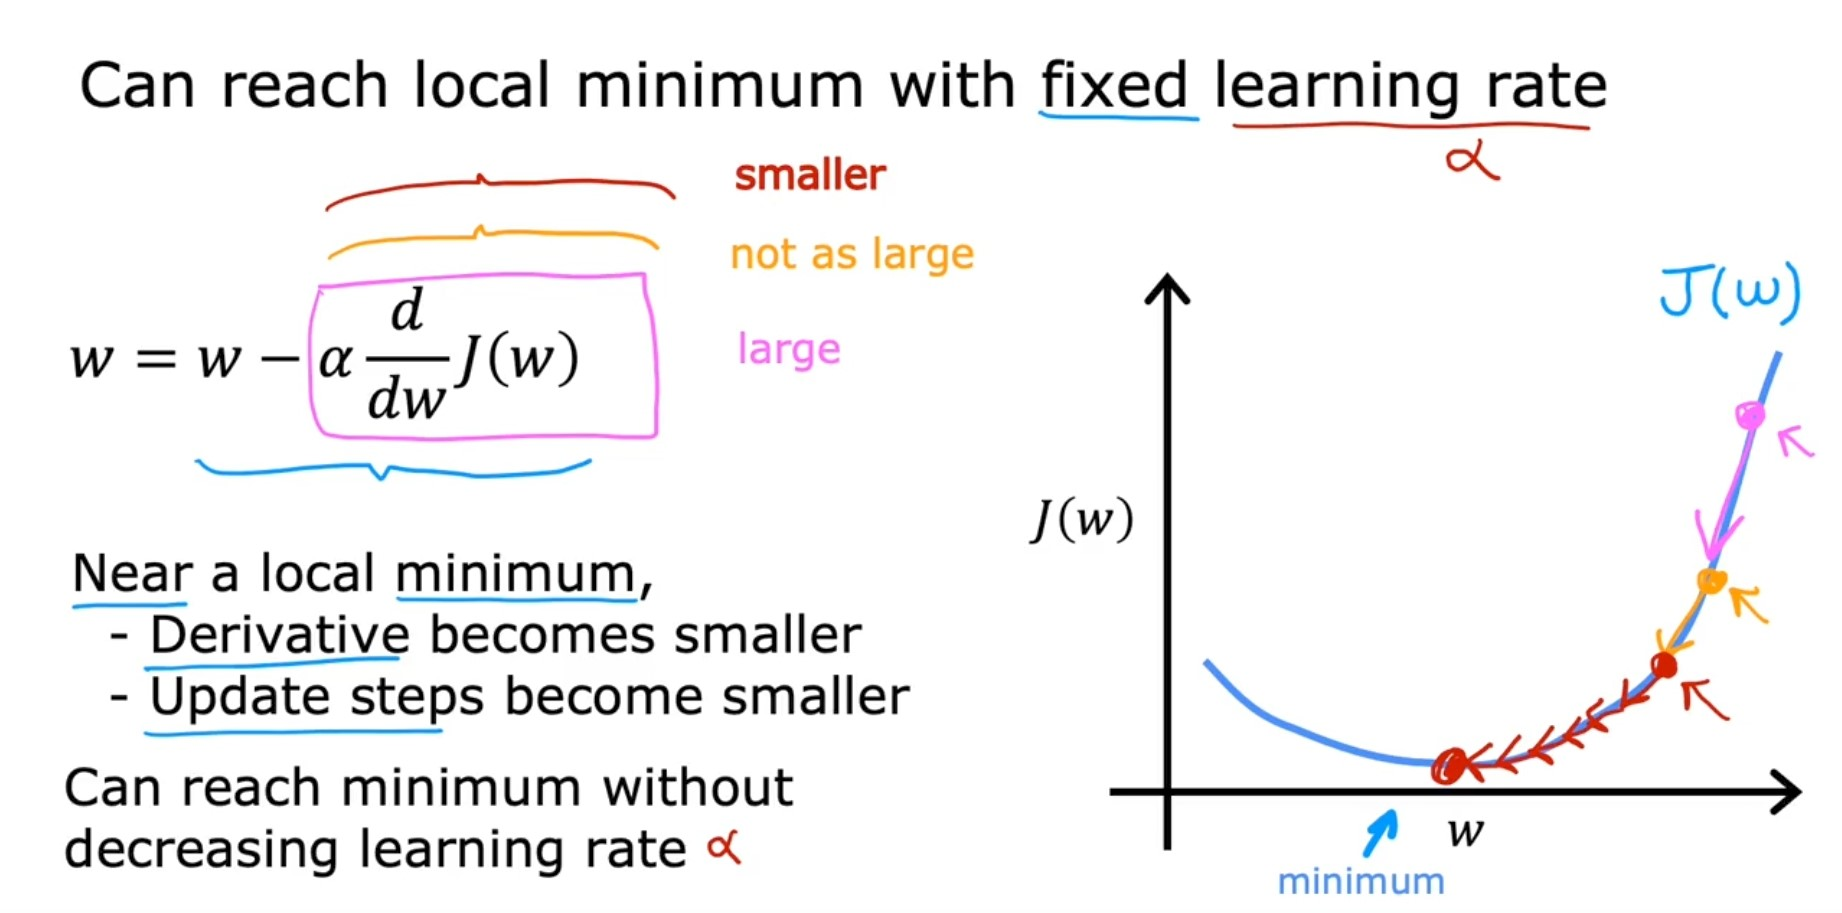
\includegraphics[width=\textwidth]{images/2.3_4}
\begin{notebox}
When near a local minima, %
the derivative become smaller, %
update will be smaller, %
so the algorithm will converge to the local minima %
without decreasing learning rate.
\end{notebox}

\section{Derivatives}
\begin{thmbox}{imporved Gradient Descent Algorithm}{algorithm_1}
\begin{align}
    w = w - \alpha \cdot \frac{1}{m} \sum_{i=1}^{m} (w \cdot x^{(i)} + b - y^{(i)}) \cdot x^{(i)} \\
    b = b - \alpha \cdot \frac{1}{m} \sum_{i=1}^{m} (w \cdot x^{(i)} + b - y^{(i)})
\end{align}
\tcblower
\begin{proof}
    \begin{align*}
        J(w, b)
        &= \frac{1}{2m} \sum_{i=1}^{m} (\hat{y}^{(i)} - y^{(i)})^2\\
        &= \frac{1}{2m} \sum_{i=1}^{m} (w \cdot x^{(i)} + b - y^{(i)})^2\\
        \\
        \frac{\partial}{\partial w} J(w, b)
        &= \frac{\partial}{\partial w} \frac{1}{2m} \sum_{i=1}^{m} (w \cdot x^{(i)} + b - y^{(i)})^2 \\
        &= \frac{1}{2m} \sum_{i=1}^{m} 2 \cdot (w \cdot x^{(i)} + b - y^{(i)}) \cdot x^{(i)} \\
        &= \frac{1}{m} \sum_{i=1}^{m} (w \cdot x^{(i)} + b - y^{(i)}) \cdot x^{(i)} \\
        \\
        \frac{\partial}{\partial b} J(w, b)
        &= \frac{\partial}{\partial b} \frac{1}{2m} \sum_{i=1}^{m} (w \cdot x^{(i)} + b - y^{(i)})^2 \\
        &= \frac{1}{2m} \sum_{i=1}^{m} 2 \cdot (w \cdot x^{(i)} + b - y^{(i)}) \\
        &= \frac{1}{m} \sum_{i=1}^{m} (w \cdot x^{(i)} + b - y^{(i)})
    \end{align*}
\end{proof}
\end{thmbox}

\vspace{2em}
\begin{notebox}
    note that the equared error cost function is \textbf{convex}, %
    so there is no local minima, %
    only global minima.\par
    so the algorithm will always converge to the global minima.
\end{notebox}

\begin{dfnbox}{Batch Gradient Descent}{batch}
    the ``batch'' in the name means that the algorithm uses all the training examples to update the parameters.\par
    some other algorithms use only a subset of the training examples. %
\end{dfnbox}